\subsection{B2}\label{B2}

In order to have just alpha numeric characters in our dataset, custom regex function was created for title, description and content columns. This would exclude special characters (such as emojis) from our data.
\begin{listing}[H]
\caption{Regex function}
\begin{minted}{python}
def apply_regex(data_frame):
    pattern = r'[^a-zA-Z0-9 ]'

    for column in ['title', 'description', 'content']:
        data_frame[column] = data_frame[column].apply(lambda x: re.sub(pattern, '', x))

    return data_frame
\end{minted}
\end{listing}

In text processing, we can remove stop words \parencite{vijayarani2015preprocessing} in order to get rid of unnecessary text. With the help of NLTK \parencite{web:Nltk} library, function bellow does this for us.
\begin{listing}[H]
\caption{Remove stopwords function}
\begin{minted}{python}
def remove_stopwords(df):
    stop_words = set(stopwords.words('english'))

    for column in ['title', 'description', 'content']:
        df[column] = df[column].apply(lambda x: ' '.join([word for word in x.split() if word.lower() not in stop_words]))

    return df
\end{minted}
\end{listing}

If we want to reduce words to its root, we can apply stemming function \parencite{jivani2011comparative}. This will be done to title, description and content columns of our dataframe.
\begin{listing}[H]
\caption{Stemming function}
\begin{minted}{python}
def apply_stemming(df):
    stemmer = PorterStemmer()

    for column in ['title', 'description', 'content']:
        df[column] = df[column].apply(lambda x: ' '.join([stemmer.stem(word) for word in word_tokenize(x)]))


    return df
\end{minted}
\end{listing}

On the other hand, if we want to apply lemmatization \parencite{plisson2004rule} in order to reduce words to their dictionary form, we can call the function bellow. It will act in a same way as stemming function.
\begin{listing}[H]
\caption{Lematization function}
\begin{minted}{python}
def apply_lemmatization(df):
    lemmatizer = WordNetLemmatizer()

    for column in ['title', 'description', 'content']:
        df[column] = df[column].apply(lambda x: ' '.join([lemmatizer.lemmatize(word) for word in word_tokenize(x)]))


    return df
\end{minted}
\end{listing}

If we want to have separate steamming and lemmatization function (that does both), we can call apply\_stemming\_and\_lemmatization. It does the same as two functions above but it is joined.
\begin{listing}[H]
\caption{Stemming and lemma function}
\begin{minted}{python}
def apply_stemming_and_lemmatization(df):
    stemmer = PorterStemmer()
    lemmatizer = WordNetLemmatizer()

    for column in ['title', 'description', 'content']:
        df[column] = df[column].apply(lambda x: ' '.join([lemmatizer.lemmatize(stemmer.stem(word)) for word in word_tokenize(x)]))


    return df
\end{minted}
\end{listing}

With topic discovery \parencite{pons2007topic}, we send in number of topics and words we want to get (defaults are set). Afterwards, data (title, description and content) is joined to list and tokenised. LdaModel (from gensim library) is used in order to generate topic models (this can be optimised with ldamulticore). At the end, dataframe of topics is returned.
\begin{listing}[H]
\caption{Topic discovery function}
\begin{minted}{python}
def discover_topics(df, num_topics=5, num_words=10):
    data = df[['title', 'description', 'content']].values.tolist()
    data = [' '.join(simple_preprocess(str(d))) for d in data]
    tokens = [d.split() for d in data]

    dictionary = Dictionary(tokens)
    corpus = [dictionary.doc2bow(doc) for doc in tokens]

    lda_model = LdaModel(corpus=corpus,\
                         id2word=dictionary,\
                         num_topics=num_topics,\
                         random_state=100,\
                         chunksize=100,\
                         passes=10,\
                         alpha='auto',\
                         per_word_topics=True)

    topics = lda_model.show_topics(num_topics=num_topics, num_words=num_words, formatted=False)

    topics_df = pd.DataFrame(columns=['topic_words'])

    for topic in topics:
        topic_id = topic[0]
        topic_words = [word[0] for word in topic[1]]
        topic_words = ', '.join(topic_words)
        topics_df = topics_df.append({'topic_words': topic_words}, ignore_index=True)

    return topics_df
\end{minted}
\end{listing}

In order to summarise articles, dataframe is passed in the function. In it, external library (gensim.summarization) \parencite{web:Gensim} is used in order to create summarization for each article which is returned at the end.
\begin{listing}[H]
\caption{Topic discovery function}
\begin{minted}{python}
def summarize_description(data_frame):
    summaries = []
    for _, row in data_frame.iterrows():
        description = row['description']
        if len(description.split('.')) == 1:
            summaries.append(description)
        else:
            summary = summarize(description, word_count=30)
            summaries.append(summary)
            
    return pd.DataFrame({'summary': summaries})
\end{minted}
\end{listing}

In the main function we can see execution of all the functions mentioned above. Data is read from CSV due to consistency. If we want to get new batch of news, get news function can be called in order to generate new data.
\begin{listing}[H]
\caption{Main function}
\begin{minted}{python}
#news = get_news(news_api_key,"bitcoin")
news_bitcoin = pd.read_csv("Data/News/bitcoin.csv", index_col=0)
news_etherium = pd.read_csv("Data/News/etherium.csv", index_col=0)
news_crypto = pd.read_csv("Data/News/crypto.csv", index_col=0)
news_cryptocurrency = pd.read_csv("Data/News/cryptocurrency.csv", index_col=0)

frames = [news_bitcoin, news_etherium, news_crypto, news_cryptocurrency]
news_all = pd.concat(frames)

# Apply regex
news_all = apply_regex(news_all)

news_stopwords = remove_stopwords(news_all)

apply_stemming(news_stopwords)[["title","description","content"]]
apply_lemmatization(news_stopwords)[["title","description","content"]]
news_stem_lemma = apply_stemming_and_lemmatization
(news_stopwords)[["title","description","content"]]

topics = discover_topics(news_stopwords, num_topics=6, num_words=10)
generate_wordclouds(news_stopwords)


plot_source_pie(news_all, n=6)
plot_publication_dates(news_all)
plot_word_count(news_stem_lemma)
\end{minted}
\end{listing}


In the news (content section) bitcoin was the most mentioned word. This matches crypto currency subreddit. Only anomaly is duplication of some words (eg crypto). 
\begin{figure}[H]
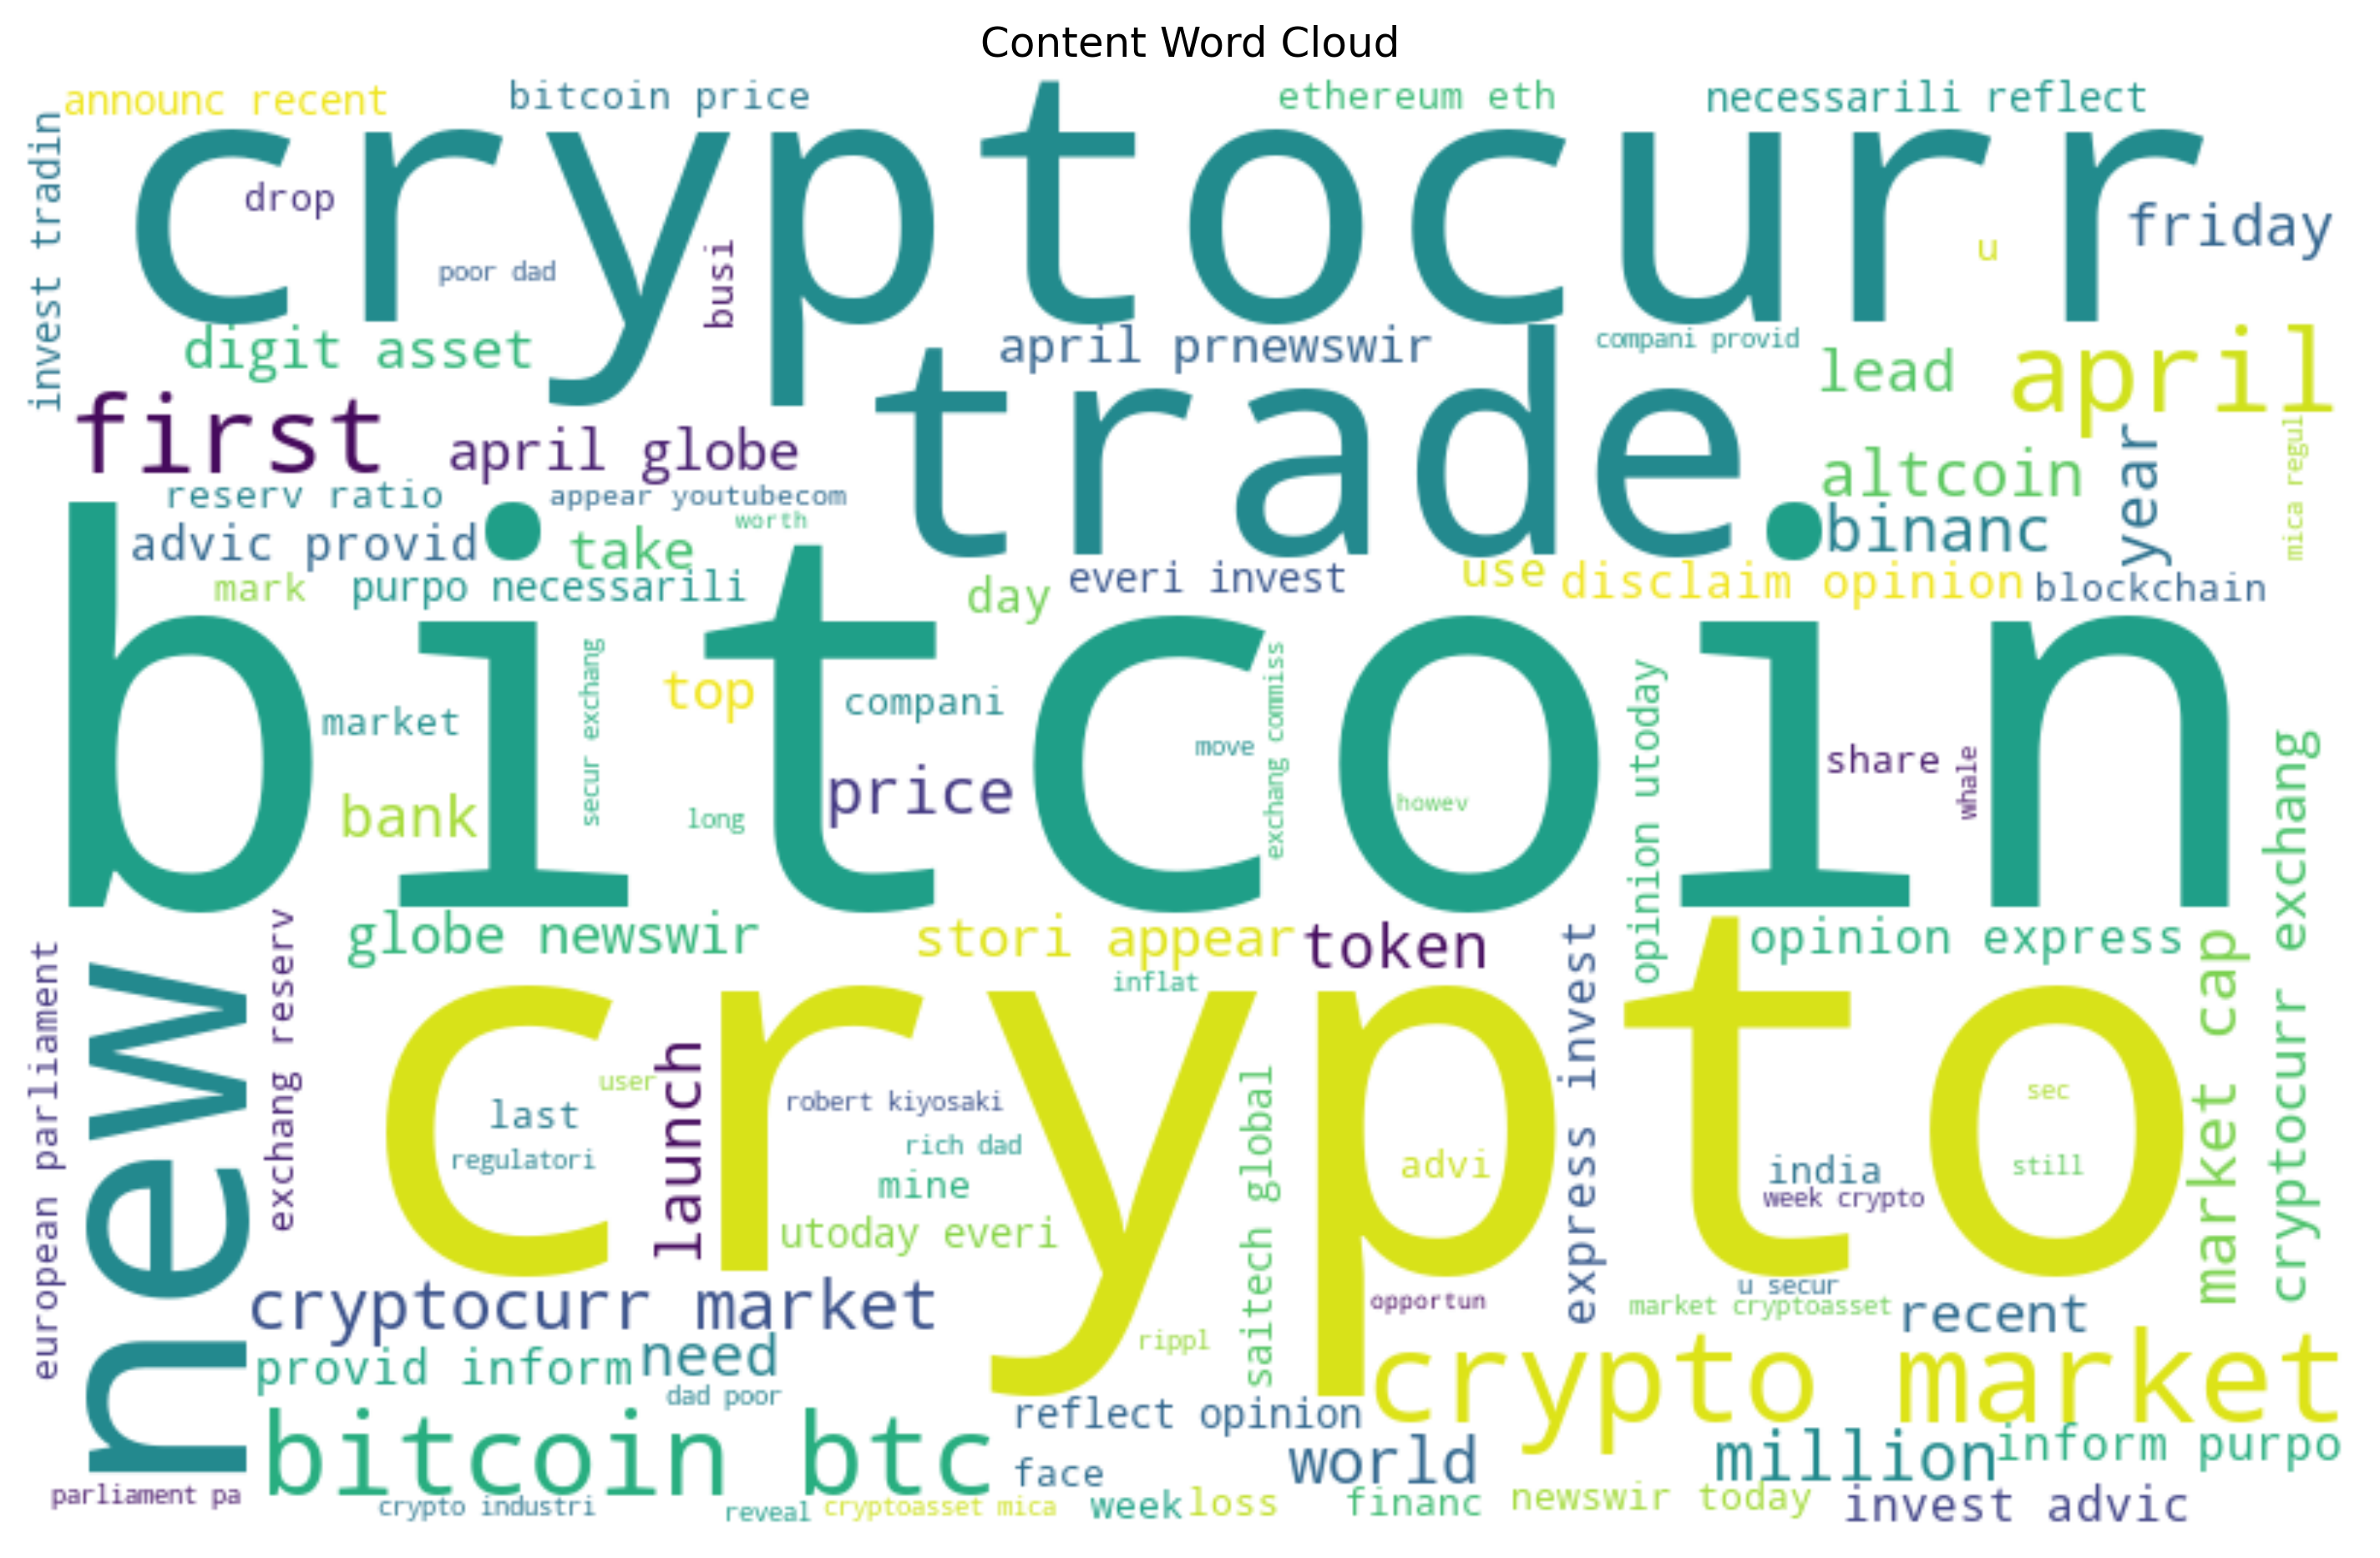
\includegraphics[scale=0.60]{img/B2/content_wordcloud.png}
\centering
\caption{News content wordcloud}
\label{fig:content_wordcloud}
\end{figure}
%\end{landscape}

Description section has similar structure, in comparison to content.This makes sense due to authors describing articles in similar styles compared to actual story.
\begin{figure}[H]

\includegraphics[scale=0.60]{img/B2/description_wordcloud.png}
\centering
\caption{News description wordcloud}
\label{fig:description_wordcloud}
\end{figure}
%\end{landscape}

Titles are much different compared to content and description worldclouds. Bitcoin and crypto are the top mentioned, but new words make an appearance (such as market). This is probably a tactical move in order to lure in new readers with the phrases known to them.
\begin{figure}[H]

\includegraphics[scale=0.60]{img/B2/title_wordcloud.png}
\centering
\caption{News title wordcloud}
\label{fig:title_wordcloud}
\end{figure}

Publication hours for most of the articles are around noon. This could simply be writers attempt to get articles out before lunch time since users tend to read after that time (and not in the evening).
\begin{figure}[H]
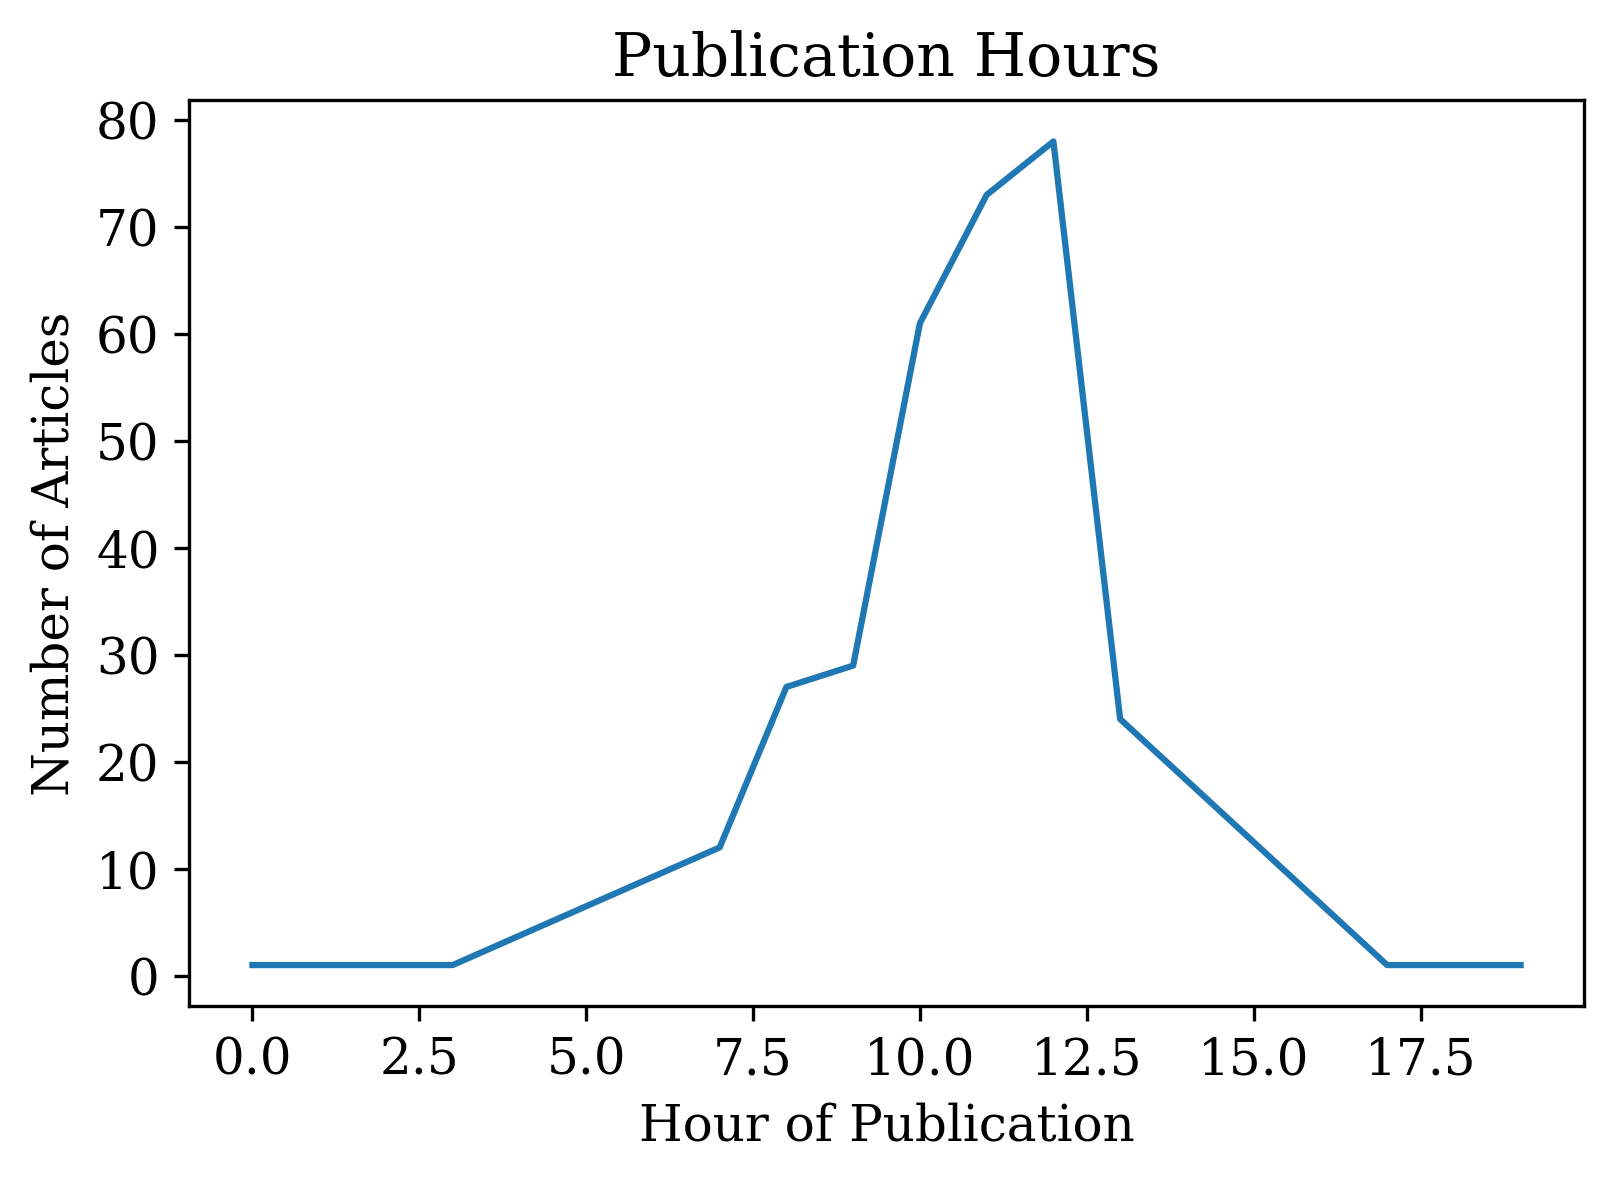
\includegraphics[scale=1]{img/B2/publication_hours.png}
\centering
\caption{Publication hours of articles}
\label{fig:publication_hours}
\end{figure}

Majority of articles are from Biztoc, a financial outlet. After further investigation, Biztoc is just a collection of articles from other sources (eg: Wallstreet Jurnal). After that, Marketscrenner and Coin desk seem to be specialising into financial news that are hosted on their site. Due to that we can say Biztoc is the biggest source of news but Marketscrenner and Coin desk are the biggest sources of original articles.
\begin{figure}[H]
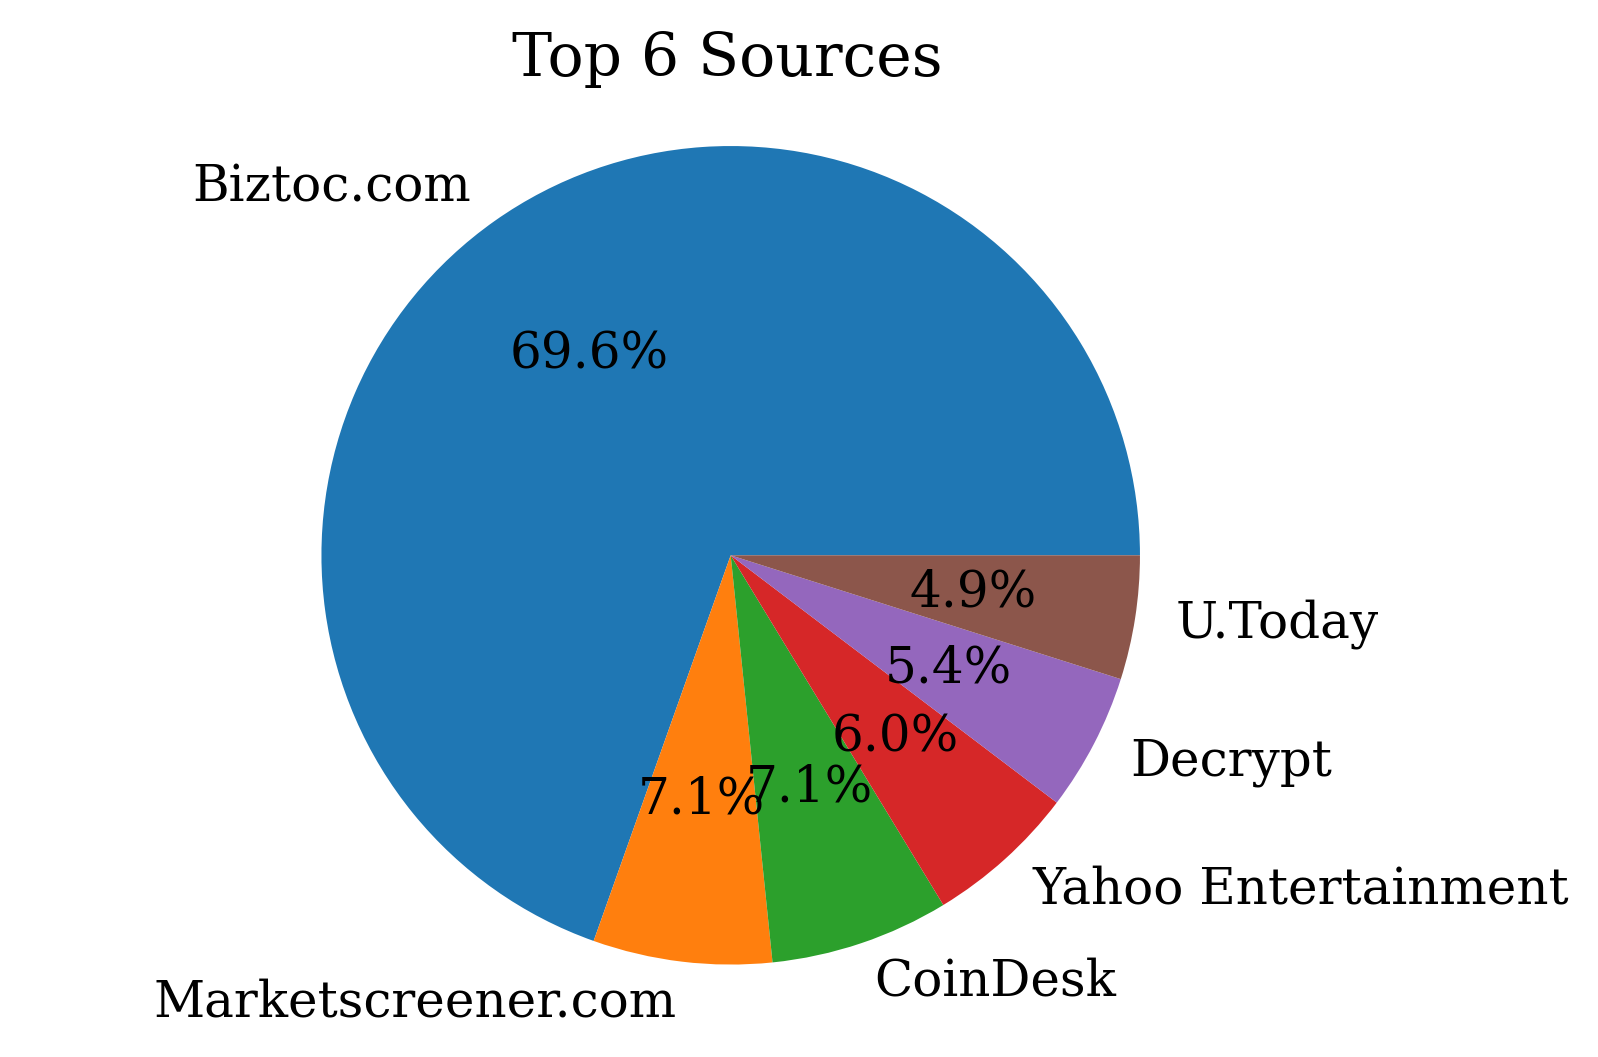
\includegraphics[scale=1]{img/B2/top_6_sources_pie_chart.png}
\centering
\caption{Top 6 sources pie chart}
\label{fig:top_6_sources_pie_chart}
\end{figure}

Creating a pie chart for most common words, we can see that crypto and bitcoin are the most popular under all of the words.
\begin{figure}[H]
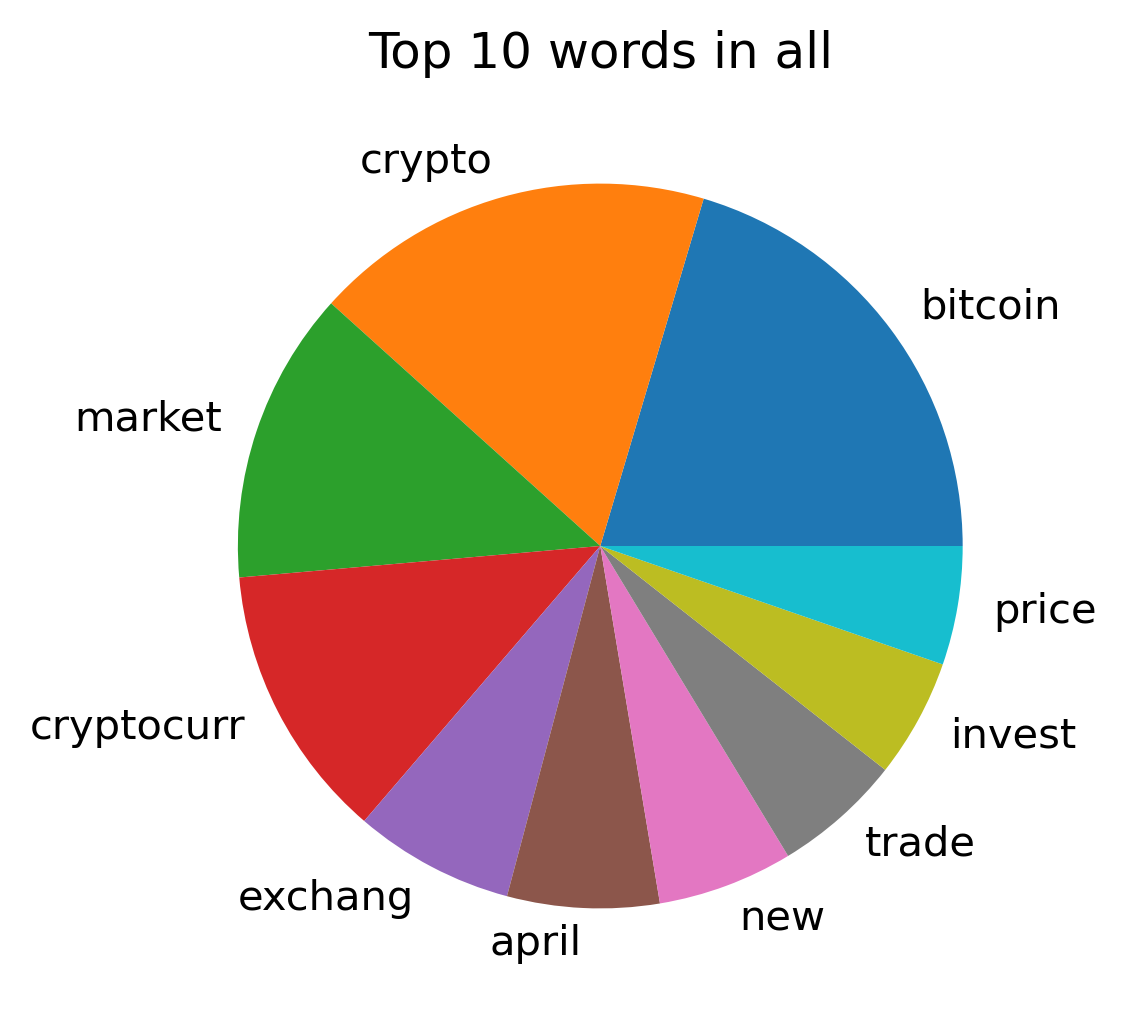
\includegraphics[scale=1]{img/B2/top_words_all.png}
\centering
\caption{Top words for all}
\label{fig:top_words_all}
\end{figure}

Content section looks similar to all, but market has a smaller portion and there is a new candidate "21". 
\begin{figure}[H]
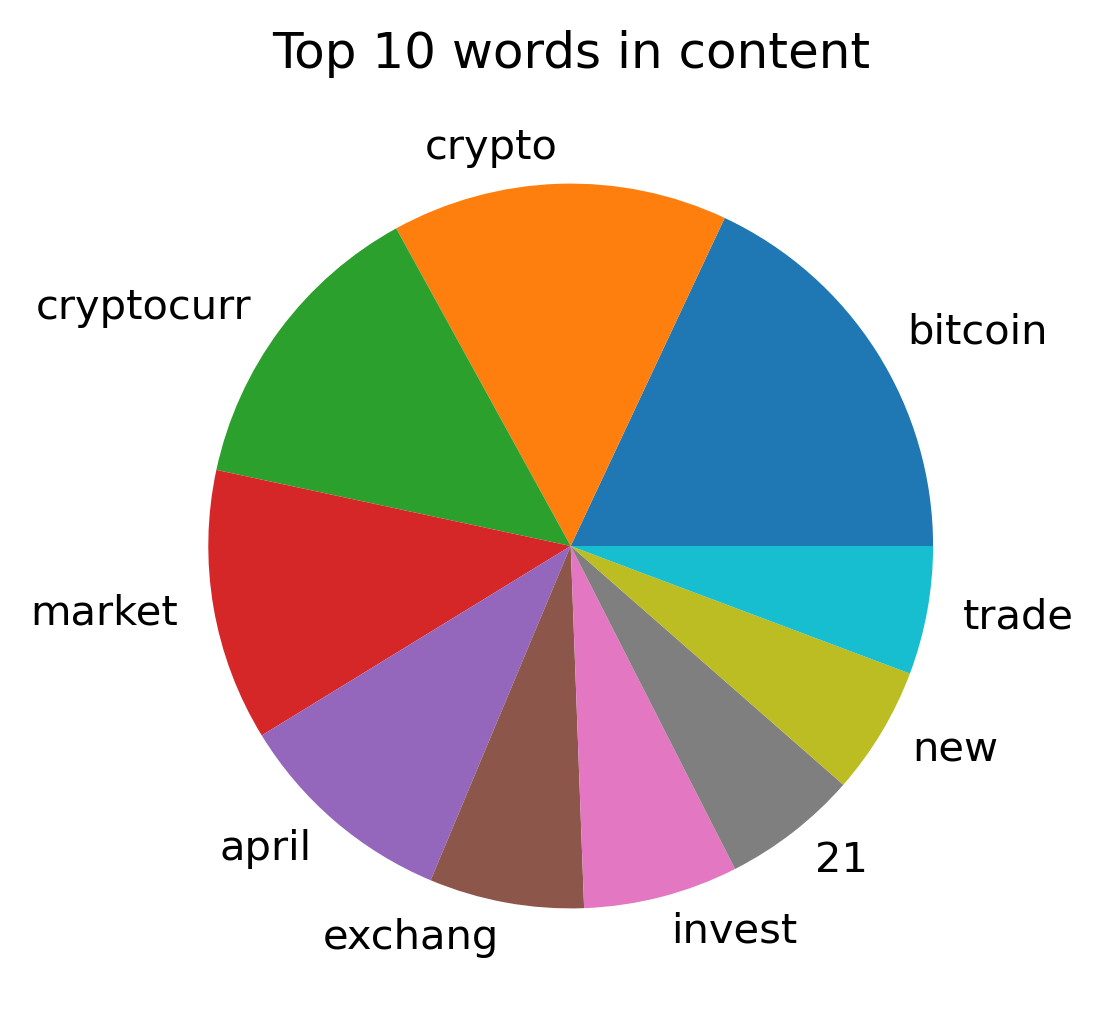
\includegraphics[scale=1]{img/B2/top_words_content.png}
\centering
\caption{Top words for content}
\label{fig:top_words_content}
\end{figure}

Description looks similar as well but it has 2023 in instead of 21.
\begin{figure}[H]
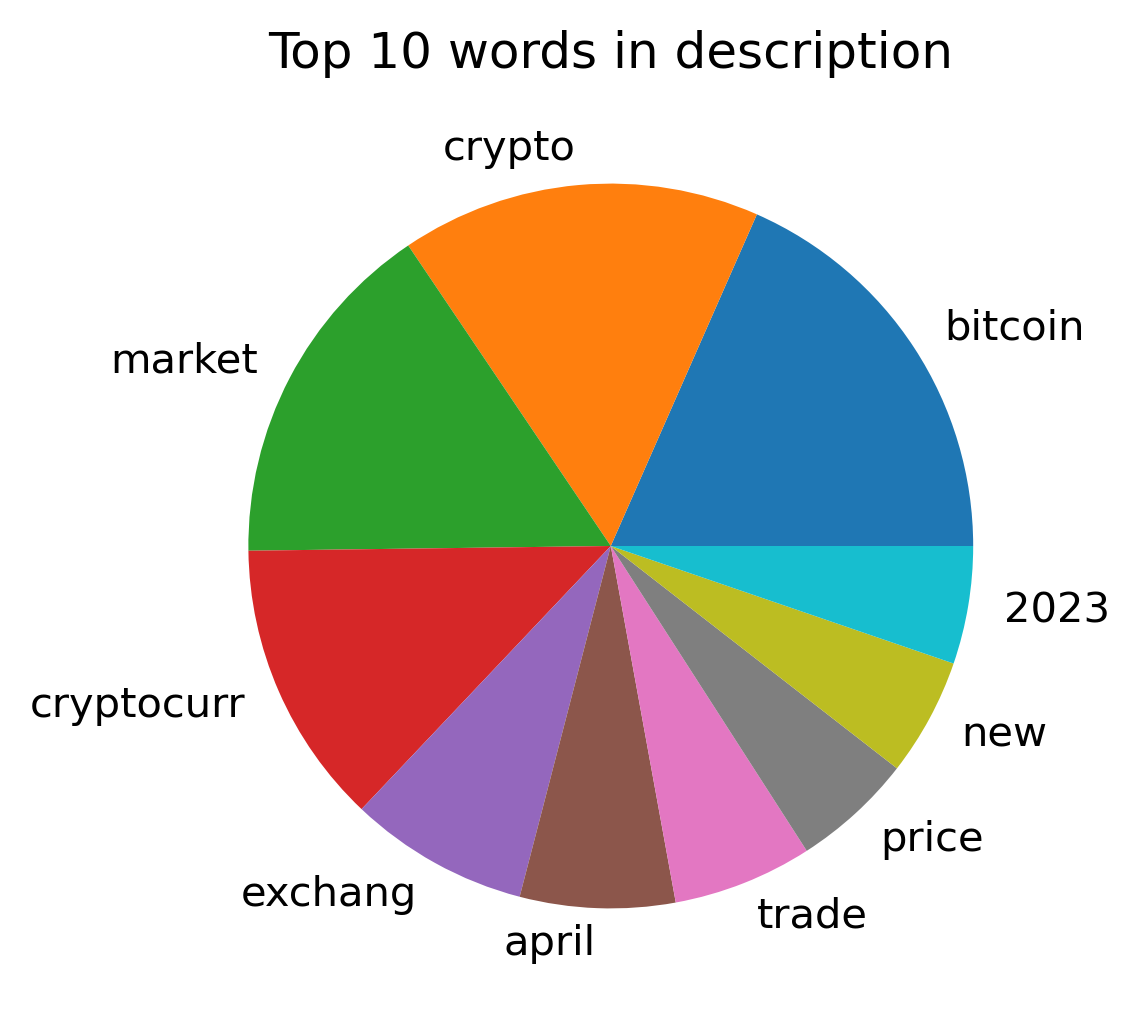
\includegraphics[scale=1]{img/B2/top_words_description.png}
\centering
\caption{Top words for description}
\label{fig:top_words_description}
\end{figure}

Title pie chart looks the most different. Although Bitcoin and crypto are on top, they share 50\% of the pie. Other well known segments from before (example: market) are much smaller.
\begin{figure}[H]
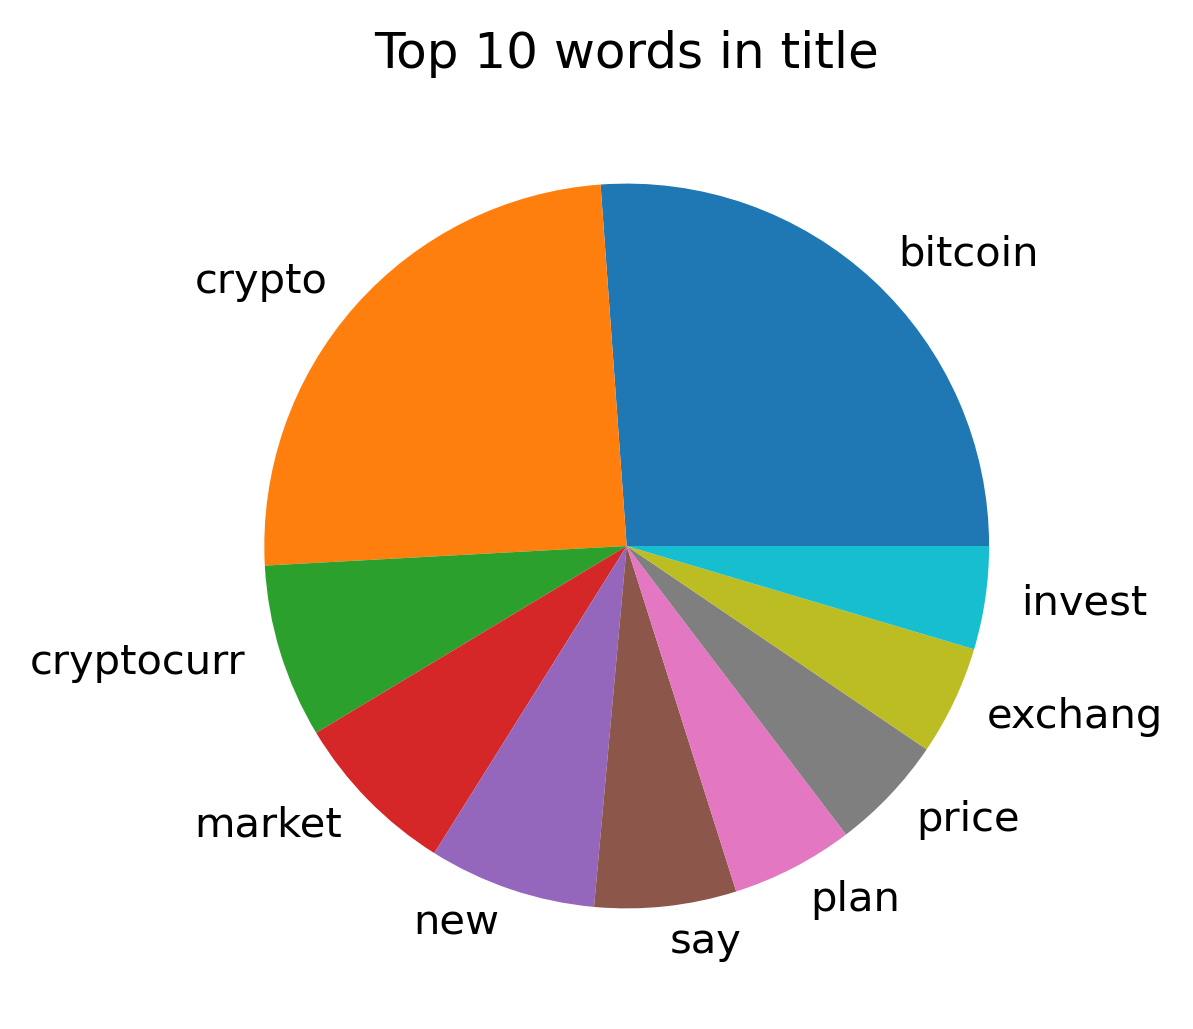
\includegraphics[scale=1]{img/B2/top_words_title.png}
\centering
\caption{Top words for title}
\label{fig:top_words_title}
\end{figure}

Looking at provided topics, we can see that our function did extract most popular topics. They seem to match search terms and its subtopics (example: energy).
\begin{figure}[H]
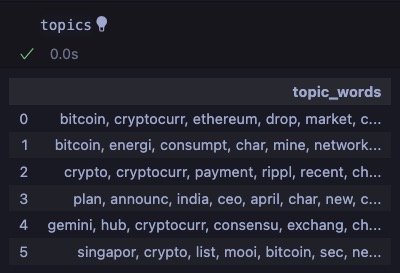
\includegraphics[scale=1]{img/B2/topics.jpg}
\centering
\caption{Article topics}
\label{fig:tArticle_topics}
\end{figure}

Summaries are not as impressive as thought. Since they have been text processed, some of the context has been removed. With that it is harder to get deeper understanding of the article. Example is article number 3, where we have upgrad downgrad, this two words don't have any special meaning. 
\begin{figure}[H]
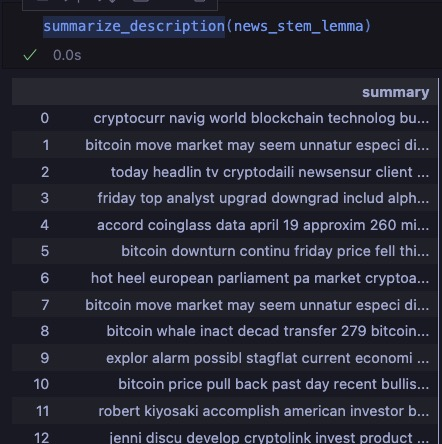
\includegraphics[scale=1]{img/B2/desc.jpg}
\centering
\caption{Article summary}
\label{fig:Article_summary}
\end{figure}